% TODO: Para cada modelo colocar como que é a entrada na forma de uma expressão matemática

Este capítulo tem como objetivo apresentar uma base teórica mínima de todos os conceitos necessários para o entendimento das demais seções deste trabalho. Primeiramente, serão explicados os conceitos básicos de uma rede neural artificial e suas diferenças em relação a uma rede neural recorrente. Subsequentemente, serão explicados os mecanismos principais de cada modelo utilizado neste trabalho.

\section{Árvores de Decisão}

% TODO: talk abiut overfitting

Árvores de decisão sobre-ajustam muito fácil no conjunto de dados por ser muito flexível e poderoso, memorizando parte do conjunto de dados. Podendo, por exemplo, criar uma árvore que cada folha corresponde a somente um elemento.

% https://towardsdatascience.com/an-implementation-and-explanation-of-the-random-forest-in-python-77bf308a9b76
 Algoritmos podem ser flexíveis e correr risco de sobre-ajuste ou ser inflexíveis e não conseguir se ajustar nos dados. Modelos flexiveis demais podem  meomorizar os dados e modelos inflexiveis presupõe informações sobre os dados.
 Árvore de decisão é flexível se não for limitar o tamanho da árvore e inflexível se vc limitar demais o tamanho da árvore. Isso é chamado de bias-variance tradeof.
 
 \begin{figure}[htbp]
    \centering
    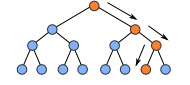
\includegraphics[scale=1.5]{monography/img/decision_tree.png}
    \label{figure:decision_tree}
    \caption[Representação do funcionamento de uma Árvore de Decisão]{Representação do funcionamento de uma Árvore de Decisão\footnotemark}
\end{figure}

\footnotetext{Corte de uma imagem de uma \textit{\acrshort{RF}} \url{https://dsc-spidal.github.io/harp/img/4-5-1.png}}

\section{\acrfull{RF}}

% TODO: checar se a tradução está correta (frase pega do abstract do artigo)
Criado por Leo Breiman em \textit{Random Forest} \cite{Breiman:2001:RF:570181.570182}, \textit{\acrshort{RF}} é um método de aprendizagem de máquina utilizado tanto para classificação quanto para regressão. Segundo o autor, o método é uma combinação de árvores de decisões onde cada árvore de decisão depende de uma amostra aleatória, sendo esta amostra independente do conjunto de dados. Além disso, todas as árvores devem possuir a mesma distribuição. 

A construção das árvores de decisão é feita utilizando o método \textit{Bagging} (\textit{\textbf{B}ootstrap \textbf{Agg}regation}), criado por Leo Breiman em \textit{Bagging Predictors} \cite{Breiman:1996:BP:231986.231989}. Este método gera várias versões de um mesmo modelo e agrega os resultados dos mesmos. As versões do modelo utilizam amostras do conjunto de dados selecionadas aleatoriamente, mas com a mesma distribuição.

% TODO: referencia apra algo que falar sobre a quantidade fixa de caracteristicas
Porém, diferente de \textit{Bagging}, \textit{\acrshort{RF}} utiliza mais uma técnica para diminuir o sobre-ajuste (\textit{overfitting}). Há uma modificação no algoritmo de criação das árvores de decisão limitando a quantidade de características (\textit{features}) do conjunto de dados que vai ser utilizada. Para selecionar a quantidade ideal de características o autor sugere utilizar de estimativas \textit{out-of-bag}, explicadas no artigo, mas é comum implementações limitarem a quantidade de características (\textit{q}) para $ \sqrt{q} $ ou $ \frac{q}{3} $.

Como \textit{\acrshort{RF}} é uma combinação de outros modelos de aprendizagem de máquina, ela pode ser classificada como um Comitê de Máquinas (\textit{Ensemble Learning}). A forma como as respostas de cada uma das máquinas são combinadas depende do problema. Para classificação pode ser usado uma votação (voto da maioria) e para um problema de regressão pode ser usado uma média dos valores, assim como mostrado na Figura \ref{figure:random_forest}.

\begin{figure}[htbp]
    \centering
    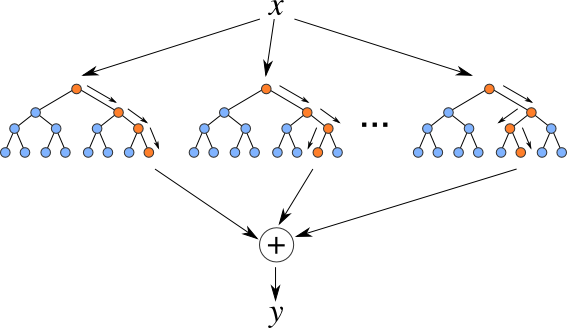
\includegraphics[scale=0.8]{monography/img/random_forest.png}
    \label{figure:random_forest}
    \caption[Representação do funcionamento de uma \textit{\acrshort{RF}}]{Representação do funcionamento de uma \textit{\acrshort{RF}}\footnotemark}
\end{figure}

\footnotetext{\url{https://dsc-spidal.github.io/harp/img/4-5-1.png}}

% RESOURCE: to learn better how random forest work (https://stackabuse.com/random-forest-algorithm-with-python-and-scikit-learn/)

\section{\acrfull{SVM}}
% TODO: adicionar examplo de uma regressão de 2 dimensões
% TODO: pegar mais referências

\textit{\acrshort{SVM}} foi criado originalmente por Vapnik nos anos 60 e foi evoluindo até se tornar o que é hoje, segundo Smola et. al. \cite{Smola03atutorial}. A ideia básica por trás do método pode ser usada tanto para classificação quanto para regressão. A aprendizagem do modelo é iterativa.

Variável C indica quanto os erros penalizam. Se for baixo, erros não serão muito penalizados e se for alto os erros serão muito penalizados

No caso da regressão, tenta-se criar uma função \(f(x)\) de forma que se \(y(x)\) é a função que perfeitamente descreve o conjunto de dados e \(\epsilon\) seja a dimensão do erro, o ideal seria \(\abs{y(x) - f(x)} \leq \epsilon \).

Além disso, \textit{\acrshort{SVM}} possuem funções \textit{Kernel}, que permitem a mudança de dimensão da entrada para alguma outra de forma rápida. Essa mudança pode aumentar ou diminuir a dimensão da entrada. Assim o modelo não tem que converter o conjunto de dados todo para tentar interpolar em outra dimensão de dados. Existem diversas funções de \textit{Kernel}, como por exemplo, Linear, Não-Linear, \textit{Radial Basis Function} e Polinomial.

Vale notar que algumas funções \textit{Kernel} possuem podem se ajustar quanto ao conjunto de dados. Funções como \textit{Radial Basis Function} e Polinomial possuem uma variável \textit{Gamma} (\(\gamma\)) para controlar esse ajuste. Essa variável determina a influência dos \textit{support vectors} no treinamento. Quanto maior o valor, menor a influência do \textit{support vectors}, quanto menor o valor, maior a influencia. Valores baixos pode levar a uma função que não se ajusta muito ao conjunto de dados, prono a sub-ajuste. Já valores altos podem levar a uma função que se ajusta muito ao conjunto de dados, prono a sobre-ajuste.

\begin{figure}[htbp]
    \centering
    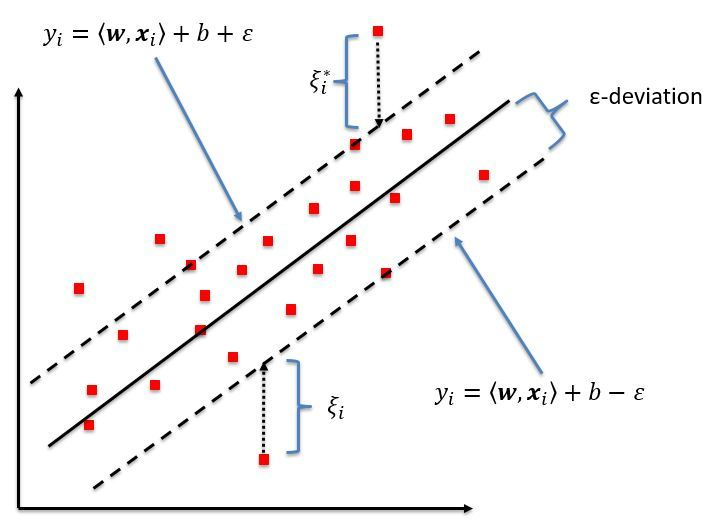
\includegraphics[scale=1.0]{monography/img/svr_example.png}
    \label{figure:support_vector_machine}
    \caption[Representação do funcionamento de uma \textit{\acrshort{SVM}}]{Representação do funcionamento de uma \textit{\acrshort{SVM}}\footnotemark}
\end{figure}

\footnotetext{\url{https://www.researchgate.net/figure/Schematic-of-the-one-dimensional-support-vector-regression-SVR-model-Only-the-points_fig5_320916953}}


\section{\acrfull{RNN}}
% RESOURCE: to explain recurrent neural networks (http://d2l.ai/chapter_recurrent-neural-networks/index.html)

% TODO: adiconar referência de onde vc tirou essa explicação

% TODO: Falar que sofre de memória curta e outros defeitos

% TODO: veja esse coisa apra explicar melhor LSTM e RNN (https://www.youtube.com/watch?v=6niqTuYFZLQ)

\textit{\acrshort{RNN}} surgiu da incapacidade de \textit{\acrfull{NN}} de levar em consideração resultados anteriores da rede para computar o resultado atual. Redes neurais artificiais comuns, ou do tipo \textit{feedforward} utilizam apenas do seu estado atual para gerar sua saída. Para exemplificar, tome como exemplo um problema de classificação, onde, a partir de uma imagem de um cachorro, ou gato, uma rede neural deva ser capaz de dizer corretamente qual animal a imagem representa. Para cada rodada de classificação, a imagem utilizada na rodada passada não importa, pois uma não tem relação direta com a outra. 

Porém, existem determinados problemas que exigem certa correlação entre os dados, como por exemplo, interpretar um documento, entender o contexto de um filme, ou avaliar a oscilação de uma bolsa de valores ao longo do tempo. Como descrito por Mtichell em \cite{mitchell1997}, \textit{\acrshort{RNN}} são mais adequadas para estas situações, pois nesse tipo de problema, dados isolados não tem tanto significado quanto o conjunto, o que exige um conceito de memória. Para simular este efeito de memória, \textit{\acrshort{RNN}} dispõe de uma arquitetura onde a saída da célula anterior é utilizada como entrada na célula seguinte, juntamente com a entrada nova atual da rede. Na Figura \ref{figure:rnn} é exemplificada a arquitetura, onde o último resultado utiliza como entrada valores resultantes das últimas execuções.

\begin{figure}[htbp]
    \centering
    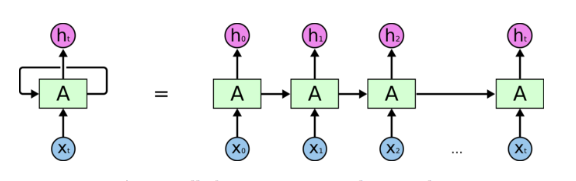
\includegraphics[scale=0.4]{rnnExample.png}
    \label{figure:rnn}
    \caption[Representação simples do conceito de um RNN]{Representação simples do conceito de uma RNN \footnotemark}
\end{figure}

\subsection{\acrfull{LSTM}}

\acrshort{LSTM} é um método proposto pela primeira vez por Sepp Hochreiter e Jurgen Schmidhuber em \cite{Sepp_1997}. Ele é utilizado para predição de informações que derivam de dados sequenciais e séries temporais, sendo possível encontrar diversos trabalhos na literatura que mostram sua eficiência quando comparado a outros métodos. Como descrito em \cite{Zainab_2018} e em \cite{Xiaolei_2015}, \acrshort{LSTM} é um tipo de \acrshort{RNN} que utiliza de estados anteriores e do estado atual da rede para gerar sua saída. Ao utilizar dos estados anteriores, a \acrshort{RNN} acaba por simular uma memória, melhorando sua capacidade de aprender. 

\begin{figure}[htbp]
    \centering
    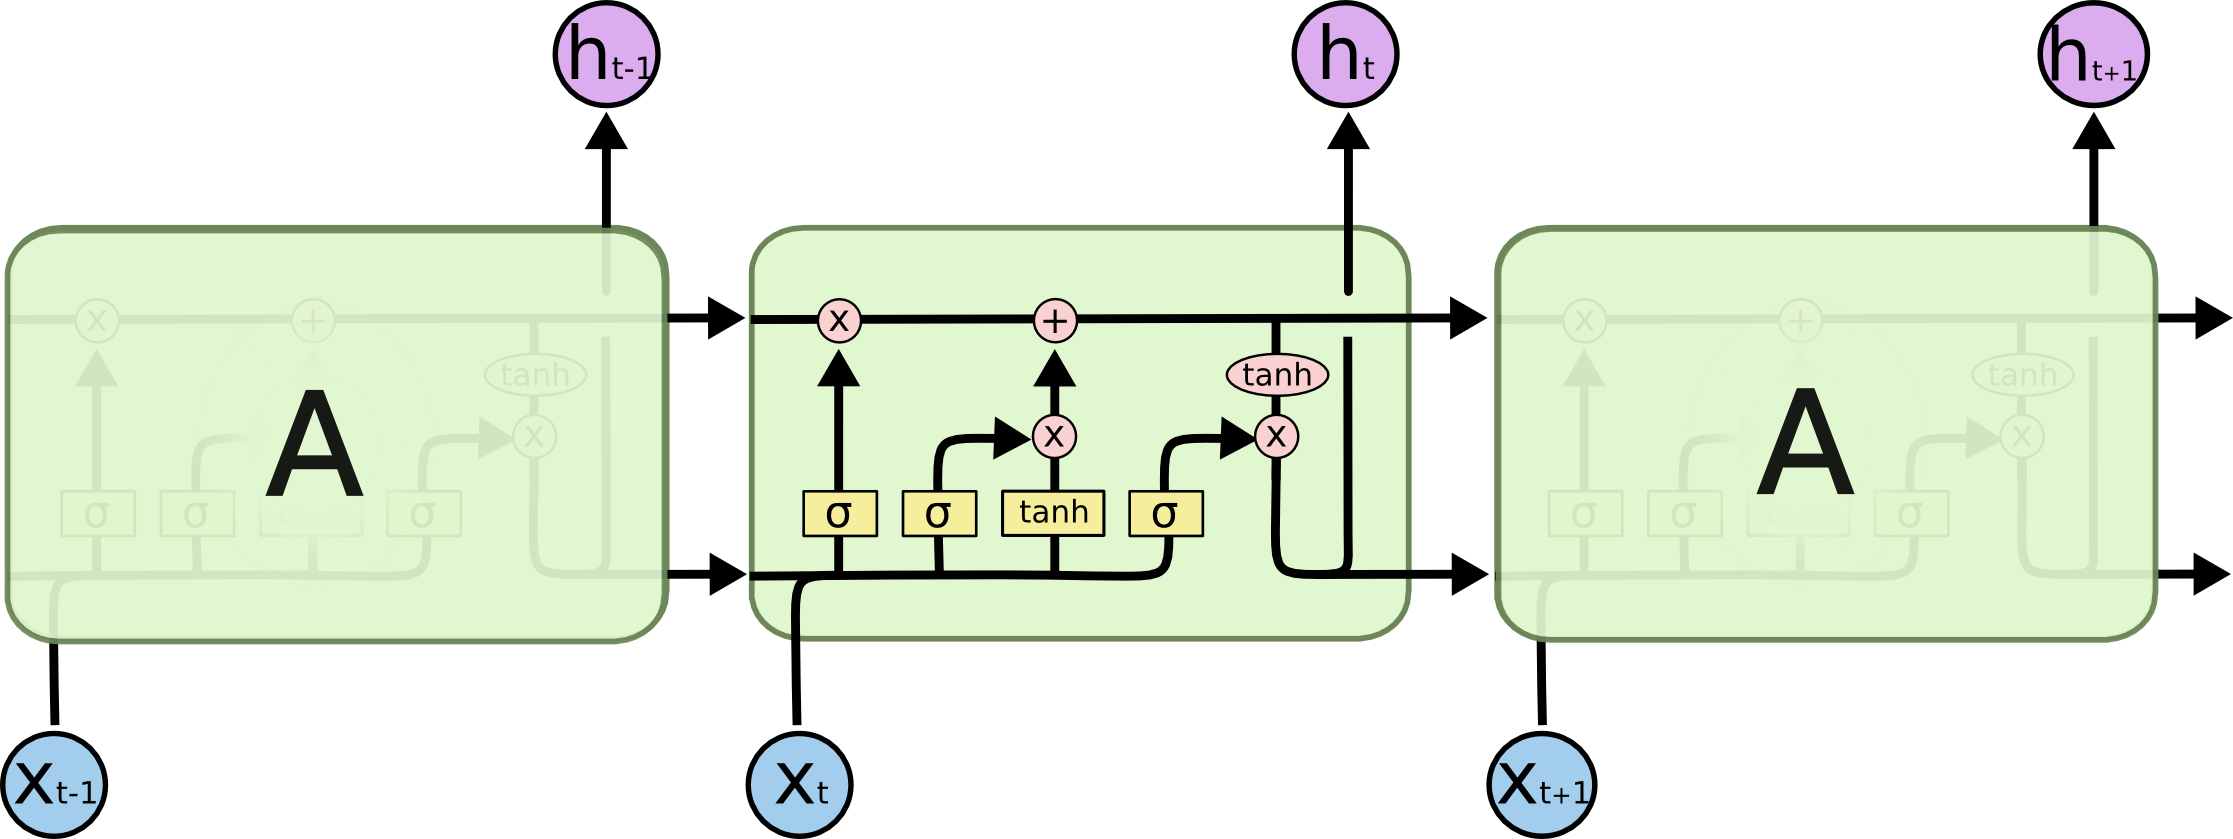
\includegraphics[scale=0.4]{lstm3.png}
    \label{figure:eixo}
    \caption[Representação de uma arquitetura LSTM]{Representação de uma arquitetura LSTM\footnotemark}
\end{figure}

\footnotetext{\url{https://colah.github.io/posts/2015-08-Understanding-LSTMs/}}

Porém, diferentemente de uma \acrshort{RNN}, o LSTM possui uma unidade chamada de célula de memória. Esta célula é capaz de perceber as características mais latentes dos dados e descartar as menos importantes. Assim, o \acrshort{LSTM} consegue manter as características mais recorrentes na rede por mais tempo que uma \acrshort{RNN} comum. 

Na célula de memória citada anteriormente, existem estruturas que são responsáveis pela característica de memória a longo prazo do \acrshort{LSTM}. A Porta de Entrada, a Porta do esquecimento e a Porta de Saída. Abaixo está explicitado como cada um deles funciona:
%TODO: melhorar explicação das portas, principalmente a porta de saída 
%TODO: colocar fórmulas que explicam como o Ct é atualizado
\begin{itemize}
  \item Porta de Esquecimento: A primeira porta de uma célula do \acrfull{LSTM} decide qual informação provinda da célula anterior vai ser descartada. Isso é feito por meio de uma função de ativação sigmoidal que retorna um número entre 0 e 1 para cada valor da célula passada, onde 0 representa total esquecimento daquela informação e 1 total preservação.
  
  \item Porta do Entrada: A segunda porta decide qual informação deve ser atualizada. Para tal decisão são utilizadas duas funções. Primeiro, uma função sigmoid decide quais valores serão atualizados. Depois uma função Tahn cria novos valores candidatos a serem utilizados na atualização.
  \item Porta de Saída: Por fim, a porta de saída efetivamente faz as alterações nos valores da célula de memória atual. Os valores candidatos decididos na Porta de Entrada são colocados no lugar dos valores que devem ser atualizados.
\end{itemize}

% TODO: Falar que podemos responder a quantidade de camadas da LSTM com o problema que RNN tem com back-propagation que o gradiente começa a diminuir exponencialmente. Mas tem que dar uma conferida melhor.

\subsubsection{Funções de ativação}

\subsection{\acrfull{GRU}}


%TODO: explicar diferenca entre porta da reinicializacao e porta da atualizacao, adicionando as fórmulas de cada uma
\textit{\acrshort{GRU}} é um tipo de \textit{\acrshort{RNN}} semelhante ao \textit{\acrshort{LSTM}} e, assim como ele, também faz uso de mecanismos chamados de Portas que possibilitam que a informação seja atualizada ou esquecida ao ser transferida de uma célula para outra. Ou seja, \textit{\acrshort{GRU}} também é capaz de guardar informações importantes na rede de maneira mais eficaz que uma \textit{\acrshort{RNN}} comum. Apesar de parecidos, \textit{\acrshort{LSTM}} e \textit{\acrshort{GRU}} possuem algumas diferenças, como pode ser visto abaixo, o \textit{\acrshort{GRU}} possui apenas duas Portas para fazer o tratamento da informação e simular o efeito de memória:

\begin{itemize}
    \item Porta da atualização: A porta de atualização tem um papel semelhante às Portas de Entrada e Porta de Esquecimento do \textit{\acrshort{LSTM}}. Nela, é decidido quais dos valores provindos das células passadas serão adicionados a rede.
    \item Porta da reinicialização: Já o portão de reinicialização decide quanto da informação vinda das células passadas será esquecido.
\end{itemize}

Por ter uma arquitetura mais simples que uma \textit{\acrshort{LSTM}}, o \textit{\acrshort{GRU}} precisa de menos tempo para ser treinado e, geralmente, de menos dados também.

\begin{figure}[htbp]
    \centering
    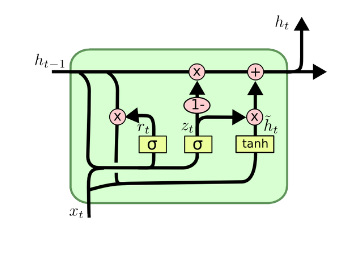
\includegraphics[scale=1.0]{monography/img/GRU.png}
    \label{figure:gru}
    \caption[Representação da arquitetura de uma GRU]{Representação da arquitetura de uma GRU\footnotemark}
\end{figure}